\section{Proposed Algorithm}

\subsection{Proposed ICP Algorithm}

\begin{algorithm}
\caption{Proposed ICP algorithm}
\begin{algorithmic}[1]
\State estimate $R_1,t_1$ using SURF
\State estimate $R_2,t_2$ using Optical Flow
\State calculate $P_1$ applying photoconsistency method with $R_1,t_1$
\State calculate $P_2$ applying photoconsistency method with $R_2,t_2$
\State set $R,t$ as $R_1,t_1$ if $P_1$ is minor than $P_2$, set as $R_2,t_2$ in other case.
\State A = edgeFilter(A)
\State B = edgeFilter(B)
\State A' $\leftarrow$ transform(A,R,t) 
\State p $\leftarrow$ closestPoints(A',B)
\State $\{R,t\} \gets$ updateTransformation(p)
\State $e_i = meanSquareError(p)$
\If {$e_i < umbral$ OR  $i > maxIterations$} 
	\State return R,t
\Else
	\State goto step 8
\EndIf
\end{algorithmic}
\end{algorithm}


In the first step the proposed algorithm uses SURF and optical flow to obtain two candidate estimations of 
R,t for the first iteration of the ICP algorithm. For each pair of consecutive RGB images optical flow 
 and SURF are applied, obtaining pairs of correspondences between both captures. 

SURF and optical flow work on the 2D image space, but using 
the 3D information from the depth map its possible to get the 3D position 
of the each pair of correspondences respect to the camera. 

Having pairs of 3D points, one point of the capture at time t and other point 
of the capture at time t + 1 its possible to obtain the rotation R and translation t
 that minimizes the distances between the correspondences. Obtaining an initial guess 
 for ICP. Then both estimations (optical flow and SURF) are compared using the photoconsistency measure, choosing 
the estimation with less photometric error.

A photoconsistency measure is used to compare the quality of the initial estimations of the sensor
 position and orientation. A good estimation of the relative transform between two captures, implies 
a small diference between the first RGB image projected using the relative transform and the second RGB 
image. Using this calculation we can detect if ICP guess is good or not.


\subsection{Complete process}

\begin{figure}[!h]
\begin{center}
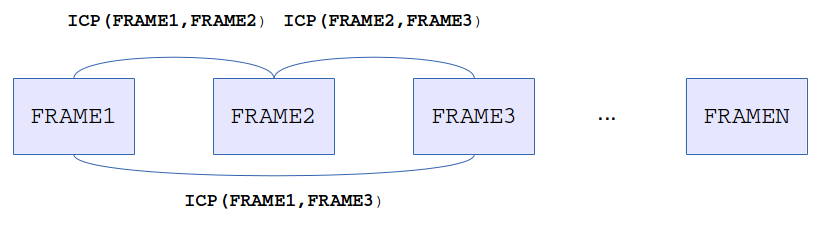
\includegraphics[scale=0.55]{images/graph_icp}
\caption{All constraints are generated using the proposed ICP.}
\end{center}
\end{figure}


The complete registration process can be described by the following algorithm:

\begin{algorithm}
\caption{General algorithm}
\begin{algorithmic}[1]
\State read prevFrame
\State globalTransf=4x4MatrixIdentity()
\State addGraphVertex(globalTransf)
\While {read frame} 
\State globalTransf=proposedICP(frame,prevFrame)*globalTransf
\State addGraphVertex(globalTransf)
\State addGraphEdge(frame,prevFrame)
\ForAll {oldFrame previous to prevFrame } 
\State detectLoop(frame,oldFrame)
\If {loopDetected}
\State addGraphEdge(frame,oldFrame)
\EndIf
\EndFor
\EndWhile
\end{algorithmic}
\end{algorithm}

Consecutive frames are readed and then both point clouds are filtered, removing plain surfaces, thus obtaining point clouds 
with a lesser amount of points. With this ICP will work on point clouds that contains around 
only 10\% or 20\% of the original points depending on the scene. But this points are highly representative for registration purposes.

Finally, the classical ICP algorithm is applied to the point clouds.

A graph is generated in the process. Adding spatial restrictions between sucesive frames and also between non-sucesive but similar 
frames. In order to reduce drift with a graph optimization approach.

\begin{algorithm}
\caption{AddGraphEdge algorithm}
\begin{algorithmic}[1]
\State [R,t] = proposedICP(framei,framej)
\State photoCons = photoConsistency(framei,framej,R,t)
\State informationMatrix=Identity6x6*photoCons;
\State graph.addEdge(i,j,R,t,informationMatrix)
\end{algorithmic}
\end{algorithm}

Note: the graph optimization algorithm internally works with quaternions instead of rotation matrices.



 






